        %auto-ignore
\section{Feature Diversity}
In this section, we show that the choice of nonlinearity and placement of nonlinearities can affect feature diversity greatly.

\subsection{Gradient Diversity}
\emph{Gradient diversity} is an important factor toward feature diversity. Observe that the gradient $\del x^l$ at $x^l$  is continuous in $l$ in the limit $L \to \infty$.  In a linear model (or the pre-nonlin model, where nonlinearity is put before the weights), this causes $\del h^l = L^{-\alpha}\del x^l$ to be very similar between neighboring blocks. As a result (because the weights $W^l$  receives an update proportional to $\del h^l \otimes x^{l-1}$), in the next forward pass, neighboring blocks contribute very similarly to the  main branch $x^l$. This leads to a waste of model capacity.

\subsection{Pre-Nonlin Leads to Poor Performance}
For example, in \Cref{fig:relu-bd1-ln0-mup-prenonlin-bm0-sweep-lr-seed}, for a relu pre-nonlin resnet (i.e. blocks are given by $W^l\phi(x^{l-1})$ instead of $\phi(W^l x^{l-1})$), we see that although Depth-$\mu$P indeed transfers hyperparameters (as predicted by our theory), the performance is dramatically worse than the post-nonlin resnet in \Cref{fig:lr_transfer}, and depth gives no performance gains beyond 8 layers. Specifically, it is because $\del h^l=L^{-\alpha}\del x^l$ like the linear case, and $\phi(x^{l-1})$ is also similar between neighboring blocks. As a result, the gradient of the weights $W^{l}$, proportional to $\del h^l\otimes \phi(x^{l-1})$, has little diversity compared to nearby blocks.

\begin{figure}
    \centering
    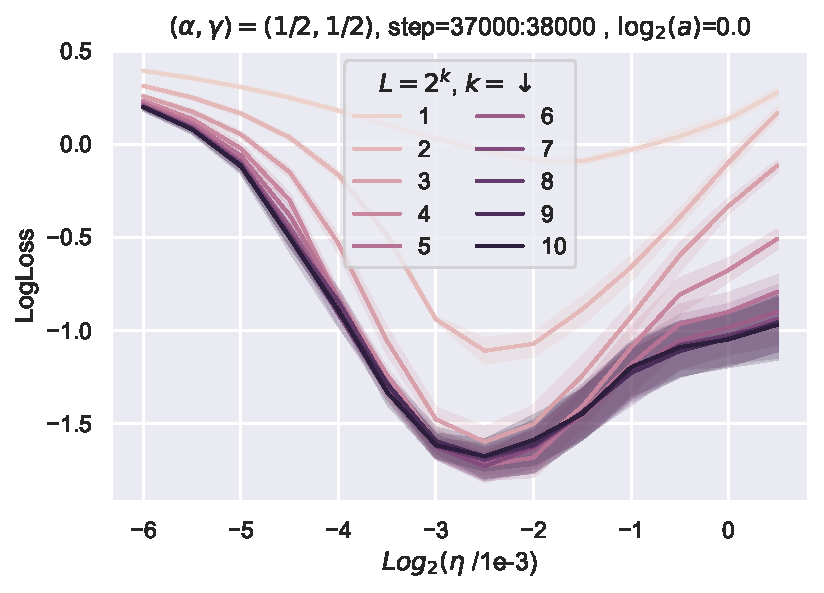
\includegraphics[width=0.4\linewidth]{fig/prenonlin_mup_37000.pdf}    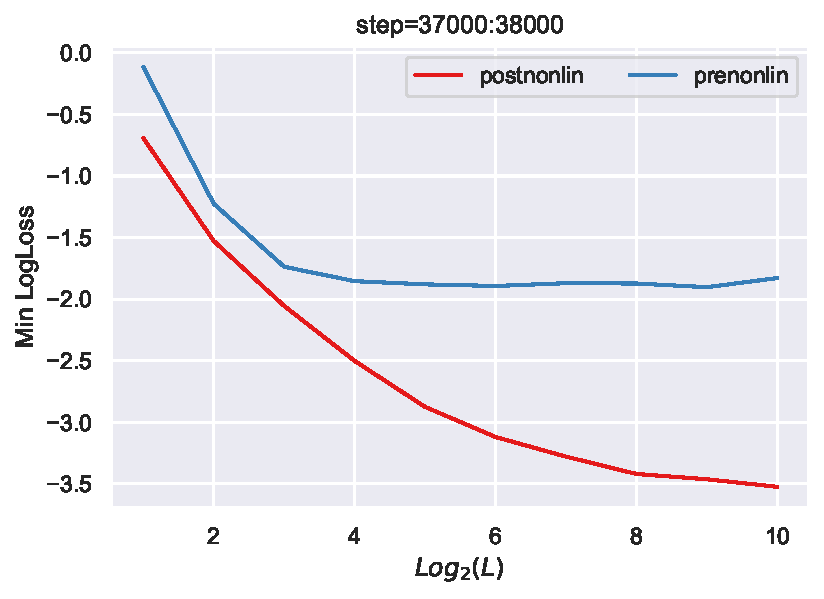
\includegraphics[width=0.4\linewidth]{fig/mup_prenonlin_vs_postnonlin_37000.pdf}
    \caption{\textbf{Pre-Nonlin Leads to Poor Performance} Although Depth-$\mu$P for prenonlin resnet indeed transfers hyperparameters (Left), depth gives no performance gains beyond 8 layers and the performance is dramatically worse than the post-nonlin resnet (Right). In right plot, the "Min LogLoss" is minimal log loss over all block multiplier and learning rate.  Networks are trained on CIFAR-10 with Adam. See \Cref{fig:lr_transfer} for more details about the setup.}
    \label{fig:relu-bd1-ln0-mup-prenonlin-bm0-sweep-lr-seed}
\end{figure}
\subsection{Maximizing Feature Diversity with Absolute Value Nonlinearity}

In a nonlinear model,  we have $\delta h^l = \delta x^l \odot \phi'(h^l)$.  Because $h^l$ is almost independent from all other $h^m, m \ne l$ in the Depth-$\mu$P limit, $\phi'(h^l)$ can serve to decorrelate the $\delta h^l$, depending on what $\phi$  is.
For example, if $\phi$ is relu, then $\phi'$ is the step function. $h^l$ is approximately a zero-mean Gaussian in the Depth $\mu$P limit, so that $\phi'(h^l)$ is approximately 0 or 1 with half probability each.
This decorrelates $\delta h^l$ much better than the linear case.
But of course, this line of reasoning naturally leads to the conclusion that $\phi' = \mathrm{sign}$ would be the best decorrelator of $\delta h^l$ and the maximizer of feature diversity (with $\phi$ among the class of positively 1-homogeneous functions) --- then $\delta h^l$ and $\delta h^m$ are completely decorrelated for $l \ne m$.

Indeed, as shown in \Cref{fig:abs-bd1-ln0-mup-bmneg1p5-sweep-lr-seed}, swapping in absolute value for $\phi$ dramatically improves the training performance of deep (block depth 1) resnets.

\begin{figure}
    \centering
    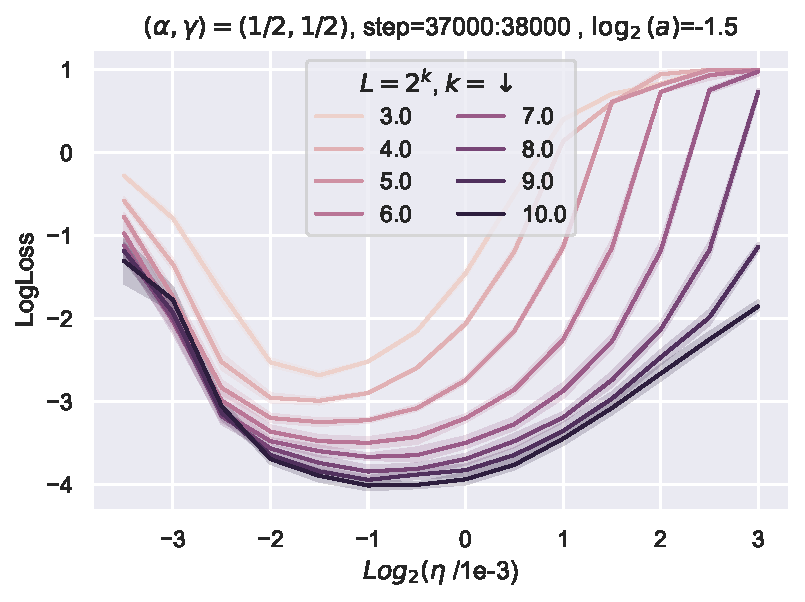
\includegraphics[width=0.4\linewidth]{fig/abs_mup_37000.pdf}
    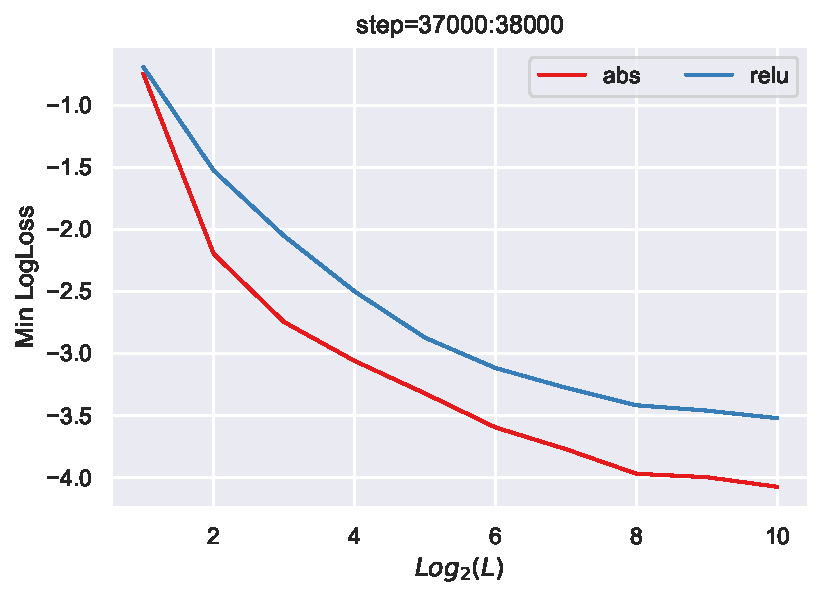
\includegraphics[width=0.4\linewidth]{fig/mup_relu_vs_abs_37000.pdf}

    \caption{\textbf{Improving performance with absolute value non-linearity}, which maximizes feature diversity. (Networks are trained on CIFAR-10 with Adam.). See \Cref{fig:lr_transfer} for more details about the setup.}
    \label{fig:abs-bd1-ln0-mup-bmneg1p5-sweep-lr-seed}
\end{figure}

In general, in lieu of absolute value,  any even nonlinearity would suffice.

\subsection{Feature Diversity is in Tension with Layerwise Linearization}

The reason that $\phi'(h^l)$ can decorrelate  $\delta h^l$ is very much related to layerwise linearization.
Recall that in Depth-$\mu$P, $h^l$ can be decomposed to a zero-mean Gaussian part $\hat h^l$ of size $\Theta(1)$ and a correction term $\dot h^l$  of size $\Theta(L^{-1/2})$ (corresponding to the decomposition $\ket{h^l} = \hatket{h^l} + \dotket{h^l}$).
$\hat h^l$ is independent from $\hat h^{m}$ for $m \ne l$ but $\dot h^l$ can be very strongly correlated to all other $\dot h^m$.
Thus, $\phi'(h^l)$ can decorrelate $\delta h^l$ precisely because $\hat h^l$ dominates $\dot h^l$, and this is also precisely the reason we have layerwise linearization.

In the $1/L$ scaling $(\alpha, \gamma) = (1, 0)$, $\hat h^l$ is on the same order as $\dot h^l$ and layerwise linearization does not occur, but also $\phi'(h^l)$ can no longer effectively decorrelated $\delta h^l$.

Once again, we remind the reader that layerwise linearization in this case is not detrimental (in this block depth 1 case) because $\hat h^l$ in fact accumulate contributions from the learned features of all previous blocks and thus strongly depends on the learning trajectory (in contrast to the (widthwise) NTK case where $\hat h^l$ is already determined at initialization).

